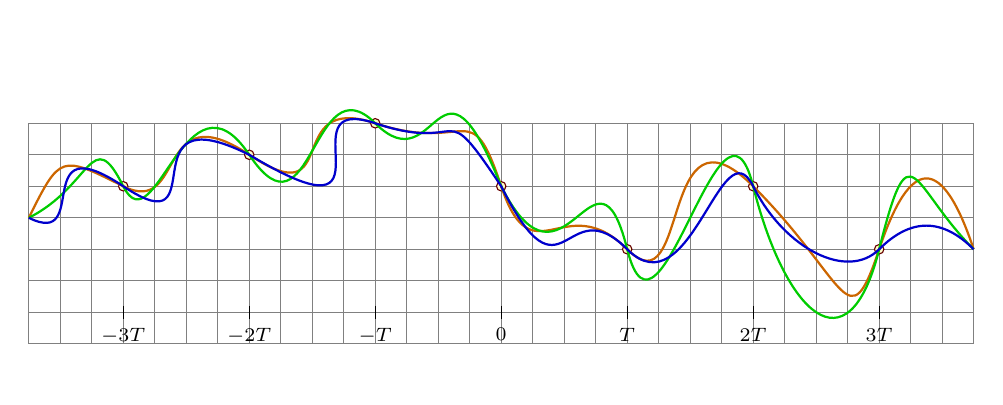
\begin{tikzpicture}[x=0.8cm, y = 0.8cm,
point/.style={circle, draw=red!40!black, fill=yellow!20, inner sep=0,  minimum size=0.12cm}
]
\draw (-7.5, 0) -- (7.5, 0);
\draw [help lines, step=0.5] (-7.5, -0.5) grid (7.5, 3);
\foreach \i/\s in {-6/{-3T}, -4/{-2T}, -2/{-T}, 0/0, 2/{T}, 4/{2T}, 6/{3T} }
{
	\draw (\i, 0.1) -- ++(0, -0.2) node [anchor=north] {\scriptsize $\s$};
}

\node [point] at  (-6,2) {};
\node [point] at  (-4,2.5) {};
\node [point] at  (-2,3) {};
\node [point] at  (0,2) {};
\node [point] at  (2,1) {};
\node [point] at  (4,2) {};
\node [point] at  (6,1) {};

\pause
\draw [thick, orange!80!black]
(-7.5,1.5)
.. controls (-7,2.5) and (-7,2.5) .. (-6,2)
.. controls (-5,1.5) and (-5.5,3.5) .. (-4,2.5)
.. controls (-2.5,1.5) and (-3.5,3.5) .. (-2,3)
.. controls (-0.5,2.5) and (-0.5,3.5) .. (0,2)
.. controls (0.5,0.5) and (1,2) .. (2,1)
.. controls (3,0) and (2.5,3.5) .. (4,2)
.. controls (5.5,0.5) and (5.5,-0.5) .. (6,1)
.. controls (6.5,2.5) and (7,2.5) .. (7.5,1);

\pause
\draw [thick, green!80!black]
(-7.5,1.5)
.. controls (-6.5,2) and (-6.5,3) .. (-6,2)
.. controls (-5.5,1) and (-5,4) .. (-4,2.5)
.. controls (-3,1) and (-3,4) .. (-2,3)
.. controls (-1,2) and (-1,4.5) .. (0,2)
.. controls (1,0) and (1.5,3) .. (2,1)
.. controls (2.5,-1) and (3.5,4) .. (4,2)
.. controls (4.5,0) and (5.5,-1) .. (6,1)
.. controls (6.5,3) and (6.5,2) .. (7.5,1);

\pause
\draw [thick, blue!80!black]
(-7.5,1.5)
.. controls (-6.5,1) and (-7.5,3) .. (-6,2)
.. controls (-4.5,1) and (-6,3.5) .. (-4,2.5)
.. controls (-1.5,1) and (-3.5,3.5) .. (-2,3)
.. controls (-0.5,2.5) and (-1,3.5) .. (0,2)
.. controls (1,0) and (1,2) .. (2,1)
.. controls (3,0) and (3.5,3) .. (4,2)
.. controls (4.5,1) and (5.5,0.5) .. (6,1)
.. controls (6.5,1.5) and (7,1.5) .. (7.5,1);

\end{tikzpicture} 